\chapter{Лінійна алгебра}
\label{chap:commentary}
\typeout{START_CHAPTER "intro" \theabspage}

Лінійна алгебра — це розділ математики, який широко використовується в науці
та інженерії. Лінійна алгебра є формою безперервної, а не
дискретної математики, тому багато людей, котрі займаються комп'ютерними науками, мають невеликий досвід роботи з нею.
Гарне розуміння лінійної алгебри є важливим для розуміння та роботи
з багатьма алгоритмами машинного навчання, особливо алгоритмами глибокого навчання.
Саме тому перед нашим вступом до глибокого навчання, ми зосередимось на необхідних поняттях лінійної алгебри.

Якщо ви вже знайомі з лінійною алгеброю, можете без зайвих вагань пропустити цей розділ. Якщо
у вас є попередній досвід роботи з лінійною алгеброю, але вам потрібна детальна довідка
стосовно основних формул, ми рекомендуємо переглянути \textit{The Matrix Cookbook} ({\color{green}Petersen and
Педерсен, 2006}). Якщо ви взагалі не знайомі з лінійною алгеброю, цей розділ
навчить вас достатньо, щоб зрозуміти цю книгу, але ми рекомендуємо вам також
зверніться до іншого ресурсу, зосередженого виключно на викладанні лінійної алгебри, наприклад
{\color{green}Shilov (1977)}. У цій главі повністю опущено багато важливих тем лінійної алгебри,
які не є важливими для розуміння глибокого навчання.

\section{Скалари, Вектоори, Матриці та Тензори}
\label{sec:definitions}

Предмет лінійної алгебри включає в себе декілька основних понять:
\begin{itemize}
\item \textbf{Скаляри}: Скаляр - це лише одне число, на відміну від більшості інших
об'єктів, що вивчаються в лінійній алгебрі, які зазвичай є масивами кількох чисел.
Скаляри записуються курсивом. Зазвичай ми даємо скалярам імена змінних у нижньому регістрі.
Декларуючи їх, ми вказуємо, що це за число. Наприклад, ми можемо сказати "Нехай $s \in \displaystyle \sR$ це нахил лінії", у випадку, якщо ми хочемо створити раціональний числовий скаляр, чи "Нехай $n \in \displaystyle \sN$ це кількість одиниць" якщо хочемо створити натуральний числовий скаляр. 
\item \textbf{Вектори}: Вектор — це масив чисел. Цифри розташовані в
певному порядку. Ми можемо ідентифікувати кожне окреме число за його індексом.
Зазвичай ми даємо векторам імена малими літерами жирним шрифтом, наприклад $x$. Першим елементом $x$ є $x_1$, другий елемент це $x_2$, і так далі. Також, нам необхідно вказати, який тип елементів знаходиться в векторі. Якщо кожен елемент це $\sR$, а сам вектор розміру в $n$ елементів, тоді вектор знаходиться в множині, утвореній декартовим добутком $\sR$ на $x$, що позначається як $\sR^{n}$. Коли ми хочемо окремо вказати елементи вектору, ми записуємо їх стовбцем огорнутим в квадратні дужки:
\begin{equation}
x = \begin{bmatrix}
x_1\\
x_2\\
x_3\\
.\\
.\\
.\\
x_n
\end{bmatrix}
\end{equation}

Ми можемо вважати, що вектори ідентифікують якусь точку в просторі, де кожен елемент визначає координату на іншій осі.

Інколи нам потрібно проіндексувати набір елементів вектору. В такому випадку ми визначаємо набір, який містить індекси і записуємо цей набір як нижній індекс. Наприклад, для того, щоб отримати доступ до елементів $x_1$, $x_3$, $x_6$, ми визначаємо набір $S = \{1, 3, 6\}$, і записуємо $x_S$. Ми використовуємо знак $-$, для того, щоб виколючити елемент з вектору. Наприклад $x_{-1}$, це вектор, який містить всі елементи $х$, крім елементу $x_1$, a $x_{-S}$ це вектор, який містить всі елементи крім $x_1$, $x_3$, $x_6$.
\item \textbf{Матриці}: Матриця це 2D масив чисел, тому кожен елемент визначається двома індексами замість одного. Зазвичай ми даємо матрицям імена, що починаються з великих літер з жирною першою буквою, наприклад $\textbf{\textit{A}}$. Якщо матриця $\textbf{\textit{A}}$ складається з раціональних чисел, має висоту $m$ і ширину $n$, тоді ми кажемо, що $\textbf{\textit{A}} \in \displaystyle \sR^{m \times n}$. Зазвичай елементи матриці ми визначаємо використовуючи ім'я матриці в курсиві, однак не в жирному шрифті, а індекси перераховані використовуючи кому. Наприклад, $A_{1,1}$ є верхнім лівим елементом $\textbf{\textit{A}}$, а $A_{m,n}$ є нижнім правим елементом матриці. Ми можемо визначити всі елементи на ветикалі з координатою $i$ пишучи ":" для горизонтальної координати. Наприклад $\textbf{\textit{A}}_{i,:}$ визначає поперечний переріз $\textbf{\textit{A}}$ з вертикальною координатою $i$. Цей поперечний переріз також відомий як $i$-товий стовбець. За схожою логікою $\textbf{\textit{A}}_{:,i}$ є $i$-товим рядком. Коли нам потрібно явно визначити елементи матриці, ми записуємо матрицю як вектор огорнутий в квадратні дужки:
\begin{equation}
\begin{bmatrix}
A_{1,1} & A_{1,2}\\
A_{2,1} & A_{2,2}
\end{bmatrix}
\end{equation}

Іноді нам може знадобитися індексувати вирази з матричними значеннями, які не є просто
однією буквою. У цьому випадку ми використовуємо нижні індекси після виразу, але не перетворюємо будь-що в нижній регістр. Наприклад $f(\textbf{\textit{A}})_{i,j}$ продокує елемент ($i$, $j$) матриці, обрахованої функцією $f$ з $\textbf{\textit{A}}$.

\item \textbf{Тензори}: У деяких випадках нам знадобиться масив із більш ніж двома осями.
У загальному випадку масив чисел, розташованих на регулярній сітці з змінною кількістю осей відомий як тензор. Позначимо тензор з назвою «A»
з цим шрифтом: \textbf{A}. Елемент \textbf{A} з координатами ($i$, $j$, $k$) позначається $A_{i,j,k}$.
\end{itemize}

Однією з важливих операцій над матрицями є \textbf{транспонування}. Транспонування матриці — це дзеркальне відображення матриці по діагоналі, котра називається
\textbf{основна діагональ} , що йде вниз і вправо, починаючи з верхнього лівого кута. Гляньте на рисунок \ref{fig:transpose} для графічного зображення цієї операції. Позначимо транспонування матриці $\textbf{\textit{A}}$ як $\textbf{\textit{A}}^T$, і це визначається таким чином, щоб
\begin{equation}
(\textbf{\textit{A}}^T)_{i,j} = \textbf{\textit{A}}_{j,i}
\end{equation}

\begin{figure}
\centering
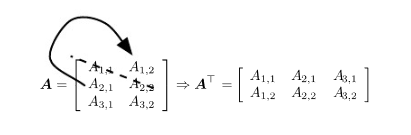
\includegraphics{transpose.png}
\caption{Транспонування матриці може бути виконано відображенням вздовж головної діагоналі.}
\label{fig:transpose}
\end{figure}

Вектори можуть виступати в ролі матриць, в якій наявний тільки 1 стовбець. Транспонування вектору створить матрицю, в якій є тільки 1 рядок. Інколи ми визначаємо вектор, записавши його елементи в текст у вигляді рядкової матриці
використовуючи оператор транспонування, щоб перетворити його на стандартний вектор-стовпець, наприклад $x = [x_1, x_2, x_3]^T$.

Скаляр можна розглядати як матрицю лише з одним записом. З цього можна побачити, що скаляр рівний власному транспонуванню: $a = a^T$.

Ми можемо додавати матриці одна до одної, однак вони повинні мати однаковий розмір. Для цього достатньо додати їххні відповідні елементи $\textbf{\textit{C}} = \textbf{\textit{A}} + \textbf{\textit{B}}$, де $\textit{C}_{i,j} = \textit{A}_{i,j} + \textit{B}_{i,j}$.

Також ми можемо додати скаляр до матриці чи помножити матрицю на скаляр. Для цього достатньо виконати відповідну операцію для кожного елементу матриці і скаляру: $\textbf{\textit{D}} = a * \textbf{\textit{B}} + c$, де $\textit{D}_{i,j} = a * \textit{B}_{i,j} + c$.

В контексті глибинного навчання, ми також можемо використовувати менш стандартні модифікації. Ми можемо дозволити додавання матриці до вектора утворюючи ще один вектор: $\textbf{\textit{C}} = \textbf{\textit{A}} + \textbf{\textit{b}}$, де $\textit{C}_{i,j} = \textit{A}_{i,j} + \textit{b}_{j}$. Іншими словами, вектор додається до кожного рядка матриці. Ця операція дозволяє уникнути створення додаткової матриці, кожен ряждок якої рівний заданому вектору. Копіювання вектору в багато місць називається \textbf{трансляцією}.

\section{Множення матриць та векторів}
\label{sec:multiplying}

Однією з найважливіших операцій, в яку залучені матриці є множення двох матриць. \textbf{Добуток матриць} $\textbf{\textit{A}}$ та $\textbf{\textit{B}}$ це третя матриця $\textbf{\textit{C}}$. Для того, щоб цей добуток існував, $\textbf{\textit{A}}$ повинна мати таку ж кількість стовбців, скільки в $\textbf{\textit{B}}$ рядків. Якщо $\textbf{\textit{A}}$ має розмір $m \times n$, а $\textbf{\textit{B}}$ має розмір $n \times p$, тоді $\textbf{\textit{C}}$ матиме розмір $m \times p$. Ми можемо записати добуток матриць просто записавши їх поруч, наприклад:
\begin{equation}
\textbf{\textit{C}} = \textbf{\textit{AB}}
\end{equation}

При чому, кожен елемент можна визначити наступним чином

\begin{equation}
\textit{C}_{i,j} =  \sum_{k}{\textit{A}_{i,k}\textit{B}_{k,j}}
\end{equation}

Зауважте, стандартний добуток двох матриць це \textit{не} просто матриця, яка містить добуток конкретних елементів. Така операція існує, і її називають \textbf{поелементним добутком} чи \textbf{добутком Гадамарда} і позначається $\textbf{\textit{C}} = \textbf{\textit{A}} \odot \textbf{\textit{B}}$

\textbf{Скалярним добутком} між векторами $\textbf{x}$ та $\textbf{y}$ однакової розмірності є матричний добуток $\textbf{x}^T\textbf{y}$. Протягом обчислення добутку матриць $\textbf{\textit{C}} = \textbf{\textit{AB}}$, ми можемо вважати, що рахуючи елемент $\textit{C}_{i,j}$, ми рахуємо скалярний добуток між $i$-товим рядком $\textbf{\textit{A}}$ та $j$-тим стовбцем $\textbf{\textit{B}}$.

We include this section as an example of some {\LaTeX} commands
and the macros we created for the book.

Citations that support a sentence without actually being used in the sentence
should appear at the end of the sentence using {\tt citep}:

\begin{quote}
Inventors have long dreamed of creating machines that think.
This desire dates back to at least the time of ancient Greece.
The mythical figures Pygmalion, Daedalus, and Hephaestus may
all be interpreted as legendary inventors, and
Galatea, Talos, and Pandora may all be regarded as artificial
life \citep{ovid2004metamorphoses,sparkes1996red,1997works}.
\end{quote}

When the authors of a document or the document itself are a noun in the
sentence, use the {\tt citet} command:

\begin{quote}
\citet{Mitchell:1997:ML} provides a succinct definition of machine learning:
``A computer program is said to learn from experience $E$ with respect to some
class of tasks $T$ and performance measure $P$, if its performance at tasks in
$T$, as measured by $P$, improves with experience $E$.''
\end{quote}

When introducing a new term, using the {\tt newterm} macro to highlight it.
If there is a corresponding acronym, put the acronym in parentheses
afterward. If your document includes an index, also use the {\tt index}
command.

\begin{quote}
Today, \newterm{artificial intelligence} (AI)\index{Artificial intelligence} is
a thriving field with many practical applications and active research topics.
\end{quote}

Sometimes you may want to make many entries in the index that all point
to a canonical index entry:

\begin{quote}
One of the simplest
and most common kinds of parameter norm penalty is
the squared $\normltwo$ parameter norm penalty
commonly known as \newterm{weight decay}.
\index{Weight decay}
In other academic communities,
$\normltwo$ regularization is also known as \newterm{ridge regression}
or \newterm{Tikhonov regularization}.
\index{Ridge regression|see {weight decay}}\index{Tikhonov regularization|see {weight decay}}
\end{quote}

To refer to a figure, use either {\tt figref} or {\tt Figref} depending on
whether you want to capitalize the resulting word in the sentence.

\begin{quote}
See \figref{fig:venn} for an example of a how to include graphics
in your document.
\Figref{fig:venn} shows how to include graphics in your document.
\end{quote}


\begin{figure}[t!]
\centering
\includegraphics{venn}
\caption{An example of a figure.
The figure is a PDF displayed without being rescaled within {\LaTeX}.
The PDF was created at the right size to fit on the page, with the
fonts at the size they should be displayed. The fonts in the figure
are from the Computer Modern family so they match the fonts used
by \LaTeX.}
\label{fig:venn}
\end{figure}

Similarly, you can refer to different sections of the book using
{\tt partref}, {\tt Partref}, {\tt secref}, {\tt Secref}, etc.

\begin{quote}
	You are currently reading \secref{sec:examples}.
\end{quote}

\section*{Acknowledgments}
We thank Catherine Olsson and \'Ulfar Erlingsson for proofreading and
review of this manuscript.


\clearpage
%%
\typeout{END_CHAPTER "intro" \theabspage}
